% shift+command+鼠标左键




\documentclass[UTF8]{ctexart} % 中文环境文件类

\usepackage{bm} % 要使用公式加粗就要调用这个包
\usepackage{color} % 要改变字体颜色就要调用这个包
\usepackage{pdfpages} % 要插入pdf就要调用这个包
\usepackage[colorlinks,linkcolor=blue]{hyperref} % 要插入超链接就要调用这个包


% 在命令行输入下面的就可以看到这些宏包的帮助文档了
% texdoc 宏包名
% 例如
% texdoc amsmath

\usepackage{amsmath} % 要使用数学公式就要调用这个包
\usepackage{amssymb}

% 注释的快捷键是command+`/'
\title{\color{red} latex体会体会-代码也有注解} % 标题
\author{zhangyifeng}

\begin{document}
\maketitle % 显示标题
\tableofcontents % 制作目录(目录是根据标题自动生成的)
	\section{Hello China} % 一级子标题
		\subsection{Hello Beijing} % 二级子标题
			\subsubsection{Hello Dongcheng District} % 三级子标题
				\paragraph{Tian'anmen Square} is in the center of Beijing
					\subparagraph{Chairman Mao} is in the center of Tian'men Square
		\subsection*{Hello Guangzhou} % 带*标题不会被编序号
				\paragraph{Sun Yat-sen University} is the best university in Guangzhou.\\
				This is my first year in UCL\footnote{University College London}. % 脚注 
				\href{http://v.youku.com/}{Youku video} % 第一个大括号写链接,第二个大括号写显示的名字
				$\sum\limits_{n = 0}^{m}$ % 求和号的上下标怎么调成正上正下方
				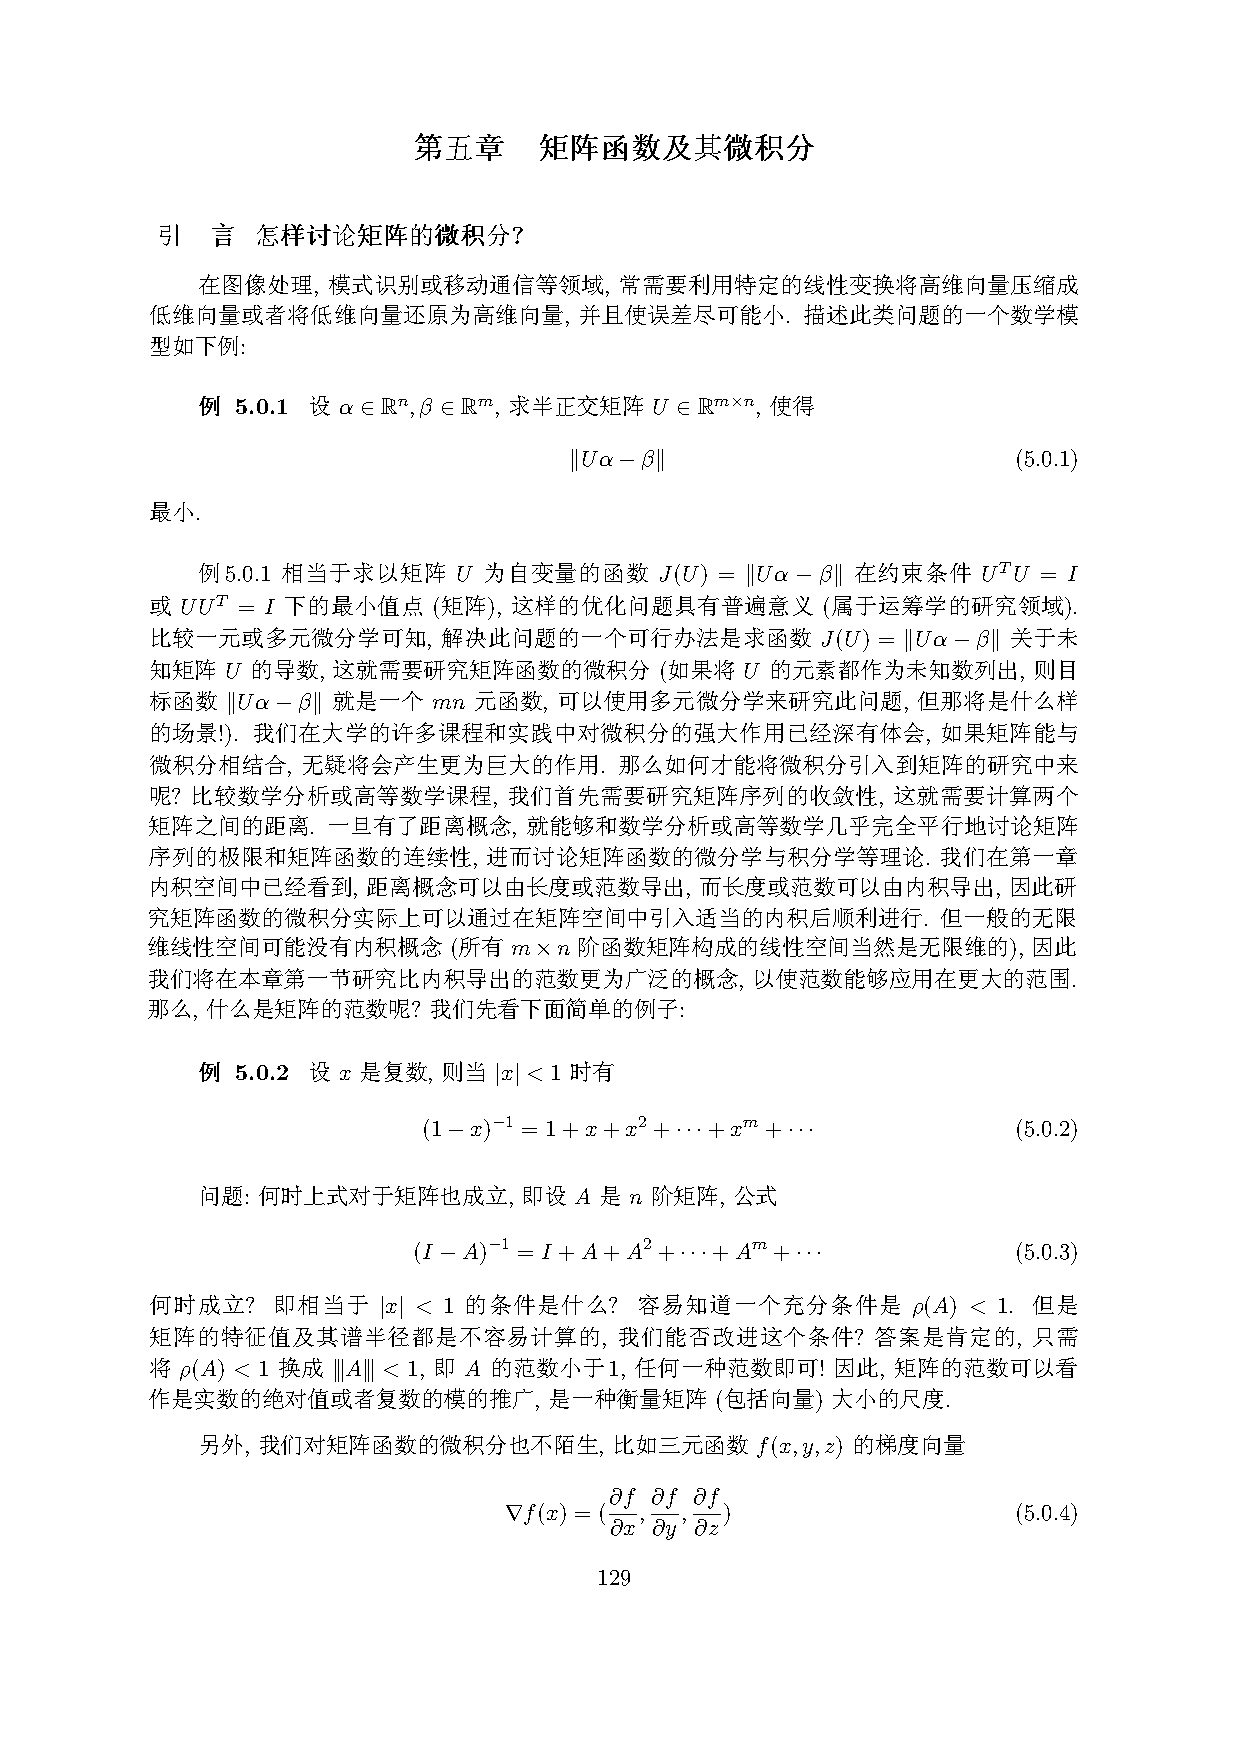
\includepdf[pages={1}]{1.pdf} % 插入1.pdf中的第一页
				% 行间公式
				\begin{equation}
				\begin{split}
				\min_{x\in \bm R^{n}}\ f(x) \\
				s.t.\  c_{i}(x)&\leq0, \ i=1,2,\cdots,k\\
				h_{j}(x)&=0, \ j=1,2,\cdots,l
				\end{split}
				\end{equation}


\end{document}